\section{Metrics}
\par{Metrics are used to evaluate and compare \acrlong{ml} models.
This text focuses on the important metrics used for multi-class classification problems.
\marginpar{
% Please add the following required packages to your document preamble:
% \usepackage{multirow}
%\begin{table}[]
    \begin{tabular}{cllll}
    \hline
    \multicolumn{1}{l}{}                &                        & \multicolumn{3}{l}{\textbf{Predicted class}}           \\
    \multicolumn{1}{l}{}                &                        & $C_0$   & $C_1$   & $C_2$                        \\ \cline{3-5} 
    \multirow{3}{*}{\rotatebox[origin=c]{90}{\parbox[c]{1cm}{\centering \textbf{Actual class}}}}   & \multicolumn{1}{l|}{$C_0$} & $a_{0,0}$ & $a_{0,1}$ & \multicolumn{1}{l|}{$a_{0,2}$} \\
                                        & \multicolumn{1}{l|}{$C_1$} & $a_{1,0}$ & $a_{1,1}$  & \multicolumn{1}{l|}{$a_{1,2}$ } \\
                                        & \multicolumn{1}{l|}{$C_2$} & $a_{2,0}$  & $a_{2,1}$  & \multicolumn{1}{l|}{$a_{2,2}$ } \\ \hline
    \end{tabular}
    %\end{table}

    \captionof{table}{Illustration of confusion matrix with 3 classes.}
    \label{tab:confusionMatrix}
    }}
\par{
    The example in table \ref{tab:confusionMatrix} will be used to introduce the different metrics.
    Table \ref{tab:confusionMatrix} illustrates a confusion matrix for a model for a problem with 3 classes ($C_j:j\in \{1;2;3\}$). 
    A model predicts the class for all observations in the set.
    The confusion matrix allows comparing these predictions against the true class\footnote{The true class is the label for this observation.}.
    $a_{0,0}$, $a_{1,1}$, $a_{2,2}$ are the correctly labelled observations. 
The predicted class corresponds to the actual class.
This is not necessarily the case for all observations. For example, $a_{2,1}$ observations with true class $C_2$ the model predicted to belong to class $C_1$.
In general, $a_{i,j}$ is the number of observations for which the model predicted $C_j$ and for which the label is $C_i$.
Based on the confusion matrix, 3 metrics can be calculated: the model \textit{precision}, the \textit{recall} and the \textit{F-score}. These are illustrated in figure \ref{fig:metrics}.
}

\begin{SCfigure}[][htb]
    \centering
    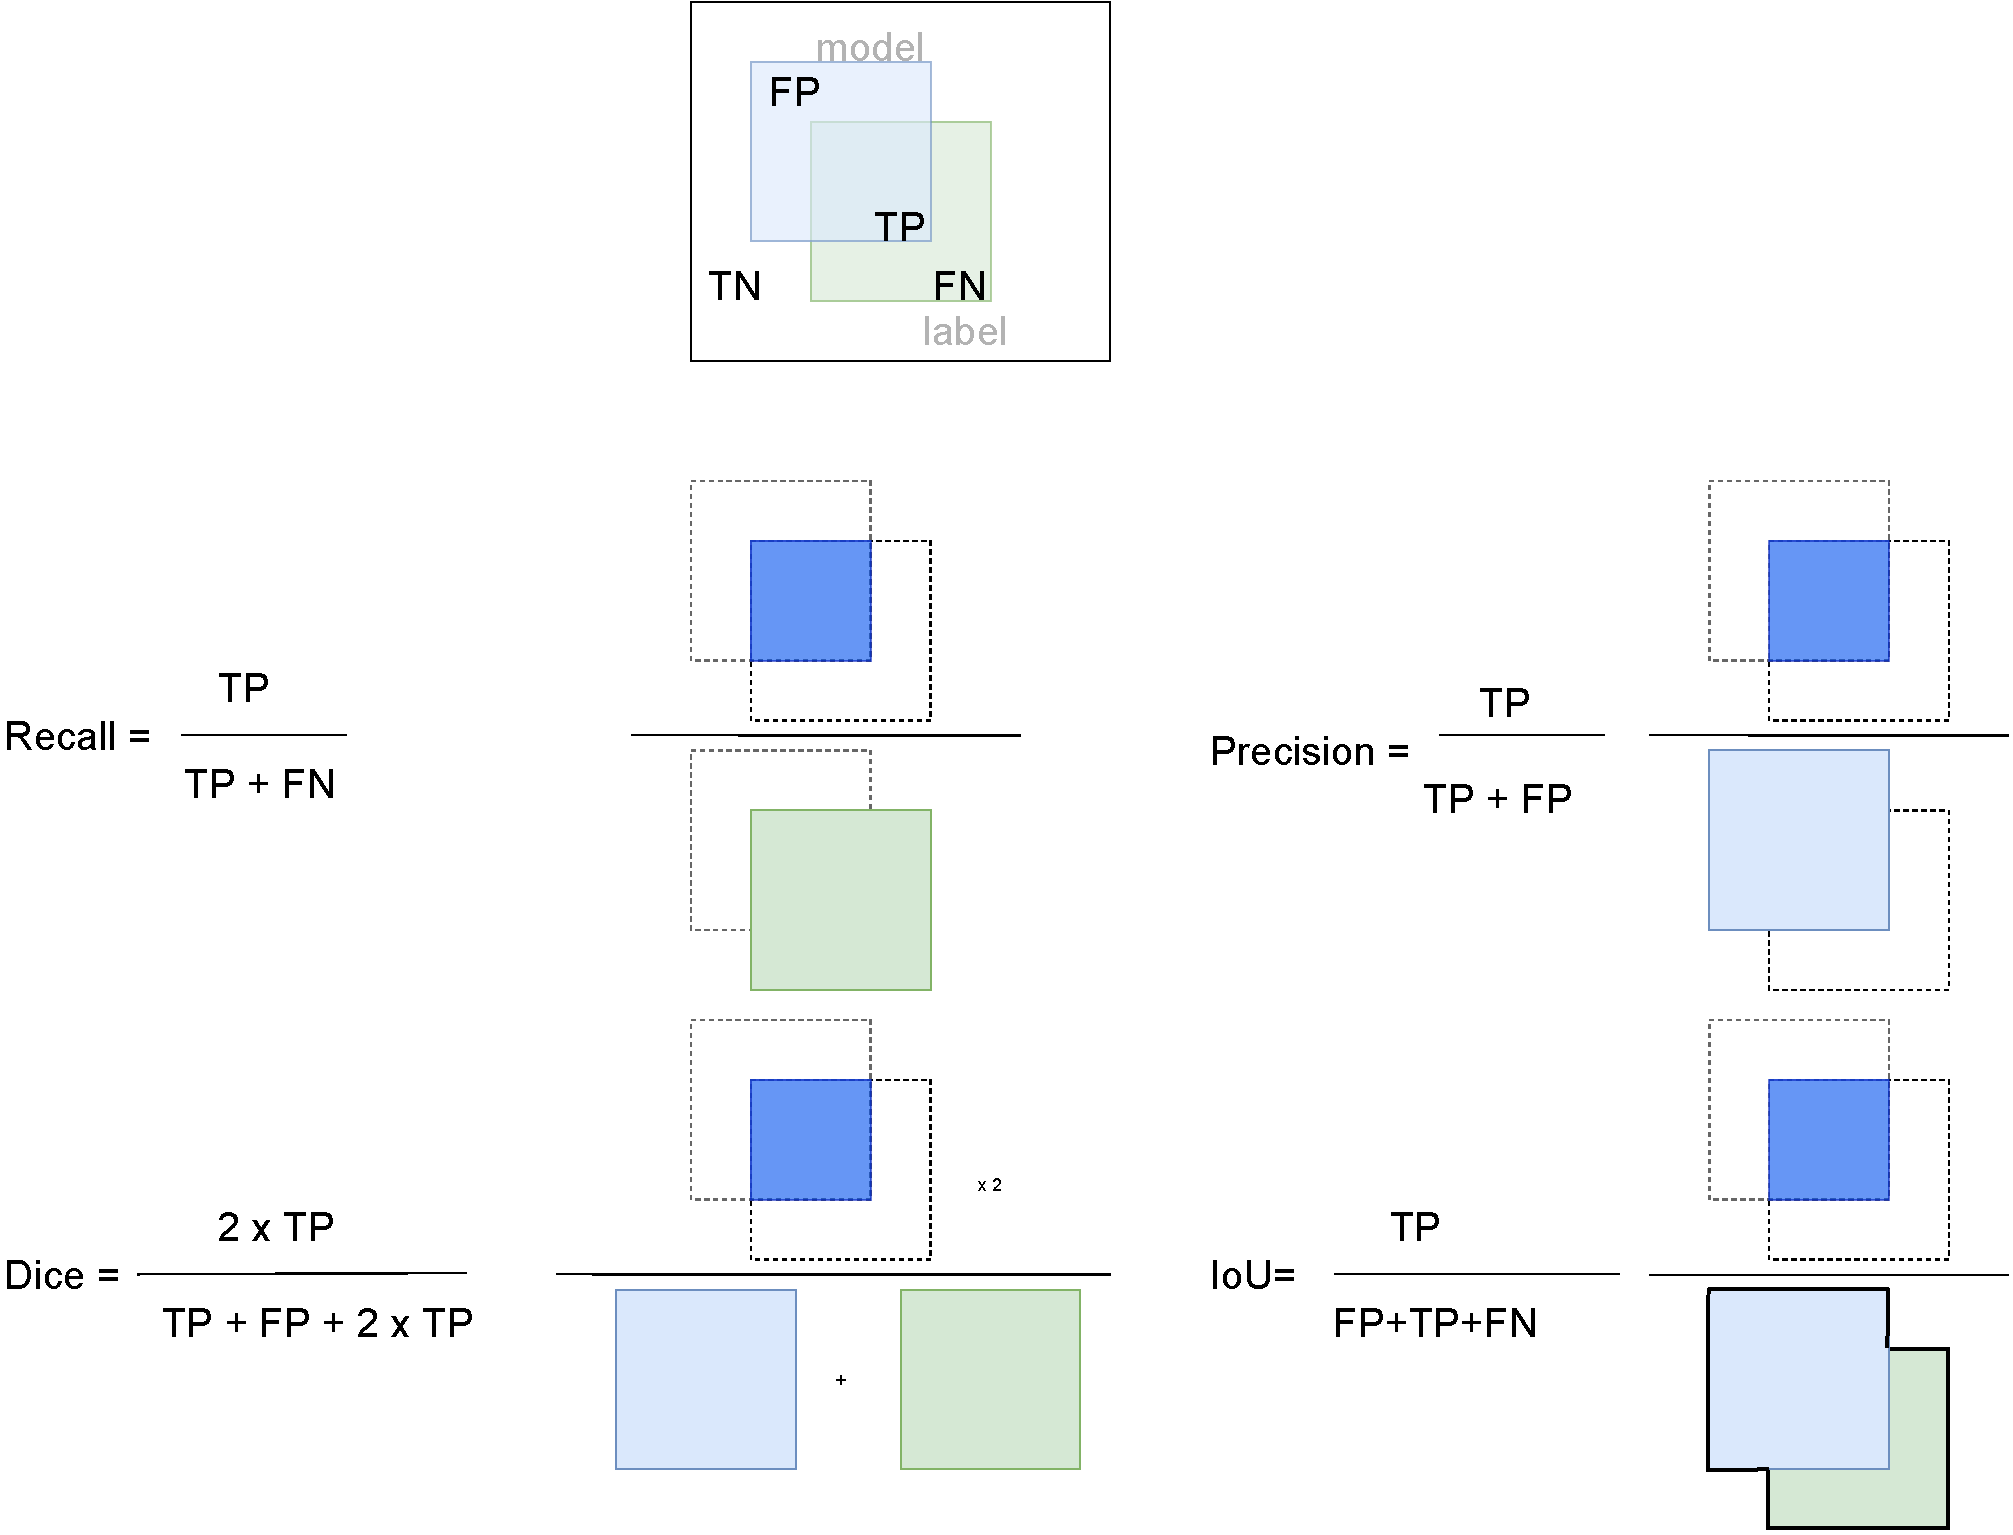
\includegraphics[width=.95\textwidth]{images/Metrics.pdf}
    \caption{Illustration of different evaluation metrics. 
    The observations for which the model correctly predicts a positive label are called the \textit{True Positive} (TP) values.
    The observations for which a positive label is wrongfully predicted are the \textit{False Positive} (FP) labels. 
    When an observation is positive, but the model fails to predict this, this is a \textit{False Negative} (FN) observation.
    On observation that is negative and is correctly predicted to be by the model is a \textit{True Negative} (TN) observation.\label{fig:metrics}
    }
\end{SCfigure}

\subsection{Class imbalance\label{sec:class_imbalance}}
\par{
    To construct an appropriate set of metrics to use for a problem, the class distribution of the dataset\footnote{
        One hopes that through a good data collection strategy, the dataset represents the population on which we ultimately want to infer.
        } needs to be taken into account.
    Imagine, for example, that one aims to segment pixels in a set of pictures where 95\% of the pixels is of the \textit{background} class and 5\% of the pixels is of the class to be segmented.
    A model can now quickly obtain 95\% accuracy by predicting every pixel as \textit{background}. This is not a metric suitable for the problem.
}
\par{
    For an evaluation metric to be valid, it has to avoid the kind this kind of pitfall.
    In this work, I investigate a problem where most of the image under investigation is \textit{background}. 
    There is about 1 pixel of each of the lumbar vertebra classes for 500 background pixels.
    The different performance metrics for the different classes are weighted with the inverse of their relative occurrence to evaluate the model's performance correctly.
}
\newpage
\subsection{Precision}
\par{
    The \textbf{precision}\footnote{the precision is also called the \textit{positive predictive value}.}, for class $i$,\footnote{
        Note that for binary classifiers (reject a null-hypothesis $H_0$ or do not reject $H_0$) the metrics for the positive class are understood to be the classifier metrics. 
        One will traditionally report the classifier precision as $\frac{TP}{TP+FP}$ without calculating the precision for the negative class where $H_0$ is not rejected.
        The binary confusion matrix clarifies the meaning of TP (True Positive) and FP (False Positive).
        \begin{tabular}{clll}
            \multicolumn{1}{l}{}                &                        & \multicolumn{2}{l}{\textbf{Pred.}}           \\
            \multicolumn{1}{l}{}                &                        & $H_0$   & $\neg H_0$                         \\ \cline{3-4} 
            \multirow{2}{*}{\textbf{Actual}}   & \multicolumn{1}{l|}{$H_0$} & $TN$ & \multicolumn{1}{l|}{$FP$} \\
                                                & \multicolumn{1}{l|}{$\neg H_0$} & $FN$  & \multicolumn{1}{l|}{$TP$ } \\ \hline
            \end{tabular}.\\
    } is the proportion of true labels $C_i$ out of all observations predicted to be $C_i$. 
    For example, the precision for class 1 in table \ref{tab:confusionMatrix} is:
    \begin{equation}
        \text{Precision}_1 = \frac{a_{1,1}}{a_{0,1} + a_{1,1} + a_{2,1}} \tag{Precision$_1$ in table \ref{tab:confusionMatrix}}
    \end{equation}.
    In general, the Precision$_i$ for class $C_i$ in a problem with $k$ classes is given by equation \ref{eq:precision_i}.
    \begin{eqnarray}
        \text{Precision}_i &=& \mathcal{P} \left( label = C_i \mid prediction = C_i \right) \\
        &=& \frac{a_{i, i}}{\sum_{j=0}^{k-1} a_{j,i}} \label{eq:precision_i}
    \end{eqnarray}
}
\par{
    One can thus calculate the precision metric for each class. 
    To calculate a precision metric for the complete multi-label classifier,
    one can either aggregate the class precisions by taking the arithmetic mean (the Macro-precision: $Precision_M$) or the weighted mean (the weighted-mean precision: $Precision_w$).
    To take the weighted mean, each precision term $Precision_i$ is weighted by the number of observations with label $C_i$. Thus, more importance is given to classes with higher occurrence. 
    \begin{eqnarray}
        \text{Precision}_M &=& \frac{\sum_{i=0}^{k-1} \text{Precision}_i}{k}  \label{eq:macro_metric}\\
        \text{Precision}_w &=& \frac{\sum_{i=0}^{k-1} \left[ \text{Precision}_i \sum_{j=0}^{k-1} a_{i,j} \right] }{\sum_{i=0}^{k-1} \sum_{j=0}^{k-1} a_{i,j} }  \label{eq:weighted_metric}
    \end{eqnarray}
}
\subsubsection{Recall}
\par{
    The \textbf{recall}\footnote{The recall is also called the \textit{sensitivity}.} is the numer of correctly predicted $C_i$ observations out of the total number of $C_i$ observations.
    For example, the recall for class 1 in table \ref{tab:confusionMatrix} is:
    \begin{equation}
        \text{Recall}_1 = \frac{a_{1,1}}{a_{1,0} + a_{1,1} + a_{1,2}} \tag{Recall$_1$ in table \ref{tab:confusionMatrix}}
    \end{equation}.
    The general expression for recall$_i$ is equation \ref{eq:recall_i}.
    \begin{eqnarray}
        \text{recall}_i &=& \mathcal{P} \left( prediction = C_i \mid label = C_i \right) \\
        &=& \frac{a_{i, i}}{\sum_{j=0}^{k-1} a_{i,j}} \label{eq:recall_i}
    \end{eqnarray}
    The weighted-mean recall and macro-recall are defined in the same way as the multi-label precision metrics, see equation \ref{eq:macro_metric} and equation \ref{eq:weighted_metric}.
}
\subsection{Dice score\label{sec:dice}}
\par{
    The objective is, of course, to build a model with both high precision and a high recall.
    There is often a trade-off to be made. 
    Increasing the recall tends to reduce the precision
    \footnote{To increase recall$_i$, you need to encourage the model to predict $C_i$. Unfortunately, this increases the probability that an observation is wrongly classified as $C_i$, thus decreasing precison$_i$.}.
    One needs to find a balance between both.
}

\par{It is useful to combine both metrics in a single new metric: the \textbf{F1-score}\footnote{The F1-score is also called the Dice-score}. This is accomplished by taking the harmonic mean
\footnote{The harmonic mean assures that F1 will always be between the values of precision and recall, but it will be closer to the lowest value. If, for example, $recall=0$ and $precision=1$, then $F1=0$.} of precision and recall.
\begin{equation}
    \text{Dice}_i = 2 . \frac{precision_i \times recall_i }{precision_i + recall_i }
\end{equation}
}
\par{
    Calculation this for Dice$_1$ in the example shows the dice score can also be described as double the intersection 
    between the points predicted as $C_1$ and the points with true label $C_1$ devided by the sum of the number of points predicted as $C_1$ and the number of points with true label $C_1$.
    \begin{equation}
        \text{Dice}_1 = \frac{2.a_{1,1}}{a_{0,1} + 2.a_{1,1} + a_{2, 1} + a_{1,0} + a_{1,2}} \tag{Dice$_1$ in table \ref{tab:confusionMatrix}}
    \end{equation}
}
\par{
    Now, there are several options for aggregation in the multi-class case:
    There are two macro F1-scores in use:
    \begin{description}
        \item[macro F1-score]: Calculate the F1-score for each class and take the arithmetic mean of the $k$ class F1-scores. As discussed in §\ref{sec:class_imbalance}, for unbalanced problems, a weighted mean can help to more accurately describe the model quality.
        \item[macro F1*-score]: Calculate the class precision and recall scores. From these class precision and recall scores, calculate the macro precision and macro recall score. 
        The macro F1*-score is given by\\ $F1_M^*=2 . \frac{precision_M \times recall_M }{precision_M + recall_M }$
        \item[weighted F1-score]: Calculate the F1 score for all classes and calculated the weighted average as is done in equation \ref{eq:weighted_metric} to calculate the weighted precision.
    \end{description}
}
The \textit{inverse} class weighted F1-score or Dice score is used to evaluate the experiment results in algorithm \ref{alg:model_training} and in part \ref{part:results} starting at page \pageref{part:results}.
The expression defining $\text{Dice}_{wi}$ is iterated below\footnote{Remark that $\sum_{j=0}^{k-1} a_{i,j}$ corresponds to all true labels that are equal to $i$.}:
\begin{equation}
    \text{Dice}_{wi} = \frac{\sum_{i=0}^{k-1} \left[ \text{Dice}_i \left( \sum_{j=0}^{k-1} a_{i,j} \right)^{-1} \right] }{\sum_{i=0}^{k-1} \left(\sum_{j=0}^{k-1} a_{i,j} \right)^{-1}} \label{eq:weighted_dice}
\end{equation}
The objective of using the inverse of the label occurrence is to increase the importance of the underrepresented classes in unbalanced data.

\subsection{Intersection over Union}

The \textbf{\acrfull{iou}}\footnote{The \acrshort{iou} is also known as the Jaccard score.} is closely related to the Dice score.
IoU is the area of overlap between the predicted segmentation and the ground truth divided by the union area between the predicted segmentation and the ground truth.
In the given example, the \acrshort{iou} score for $C_1$ is:
\begin{equation}
    \text{IoU}_1 = \frac{a_{1,1}}{a_{0,1}+a_{1,1}+a_{2,1}+a_{1,0}+a_{1,2}} \tag{IoU$_1$ in the table \ref{tab:confusionMatrix}}
\end{equation}

In general, the class specific \acrfull{iou} for class $C_i$ is given by:
\begin{equation}
    \text{IoU}_i = \frac{a_{i,i}}{\sum_{j=0}^{k-1} a_{i, j} + \sum_{j=0}^{k-1} a_{j,i} - a_{i,i}} 
\end{equation}

Again, a macro IoU score can be calculated by taking the arithmetic mean of the class IoU scores.

\subsubsection{Classifier accuracy}

Finally, the classifier accuracy is defined as the proportion of the observations that are correctly classified:
\begin{equation}
    \text{accuracy} = \frac{a_{0,0} + a_{1,1} + a_{2,2}}{\sum_{i=0}^{2} \sum_{j=0}^{2} a_{i,j}   } \tag{table \ref{tab:confusionMatrix} classifier accuracy}
\end{equation}

In general, the classifier accuracy is defined by 
\begin{equation}
    \text{accuracy} = \frac{\sum_{i=1}^{k-1}a_{i,i}}{\sum_{i=0}^{k-1} \sum_{j=0}^{k-1} a_{i,j}   } 
\end{equation}


